\documentclass[11pt,a4paper]{report}
\renewcommand\thesection{\arabic{section}}
\usepackage[utf8]{inputenc}
\usepackage{amsmath}
\usepackage{amsfonts}
\usepackage{amssymb}
\usepackage{graphicx}
\title{CS571 Project Report (P2)}
\author{T21016}
\date{23/11/2021}
\begin{document}
\maketitle
%Notes:
%\begin{enumerate}
%\item The report should be about 4-5 pages. You can use more pages if you need to include plots etc.
%\item Do a spell check.
%\item Do not include any source code in the report.
%\end{enumerate}
\section{Summary}
\ Pitch is the fundamental frequency of an harmonic pattern of a signal.


\  The goal of this project is to use Python to automatically compute the pitch of an audio signal. To do this, I must first prepossess the signal and extract the speech portion from it; for this, we employed energy-based segmentation. After that, I have utilised auto-correlation, which determines how similar a signal is to itself as a function of time lag. This method falls under the time domain technique of calculating pitch. There are several superior approaches available, such as the average magnitude difference function (AMDF), Cepstrum Methods, and the frequency domain method: harmonic analysis. This project focuses solely on ACF short-term analysis.


\ So to achieve our objective of pitch estimation we will first develop our algorithm and test it with different sound wave also we will discuss the limitation of this project finally.
 
\section{Introduction}
Pitch estimation from a sound is a difficult problem since speech signals are quasi periodic waves with a mix of harmonic functions, and there are noise constraints. So we're looking for a way for a computer to automatically discern the pitch that people perceive from sounds. If we can create an algorithm that can provide us with a decent grasp of pitch, we may use it to solve a variety of difficulties, such as automatically transcribing melodies, algorithmic interpretation of speech with tonal variation, and voice sentiment analysis.

\section{Solution}
\ Now that we've identified the issue, let's look at the remedy I'm proposing.
The method we are employing is a time domain approach known as auto-correlation. As a naïve approach, it will have certain issues that will be explained further down, but for now, let's focus on how we can retrieve the pitch by utilising the auto-correlation function.
Now the issue is, what precisely is auto-correlation?
The solution is simple: auto-correlation is a subset of cross-correlation that measures the similarity of two signals.
Mathematically for two discrete finite duration signal $x(n)$ and $y(n)$

\begin{equation} r_{xy}(l) =  \sum_{n=\infty}^{\infty} x(n+l)y(n)   \end{equation}


\
\ 
\  
\    
\ where $l$ represent the delay variable.Now that we have seen the cross-correlation same way we have the expression for the auto-correlation.


\begin{equation} r_{xx}(l) =  \sum_{n=\infty}^{\infty} x(n+l)x(n)   \end{equation}


\ Now to understand how auto-correlation function estimates the pitch of a signal let's generate a simple discrete time signal . 
\ EXAMPLE
\[ x(n)  = sin(2\pi 10 n) \]

\ this $x(n)$ sinusoidal signal will repeat itself $10$ time in one second , see the plot below

\begin{figure1}
	\centering
	\begin{subfigure}
		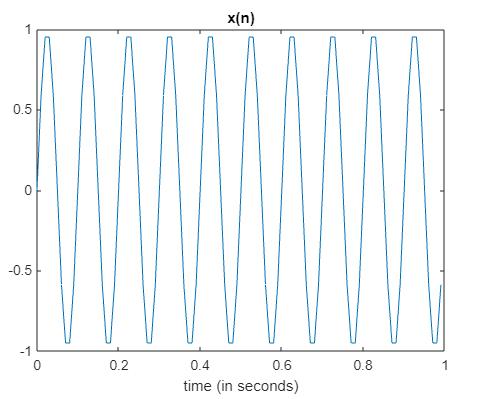
\includegraphics[width=\textwidth]{Untitled.png}
		\caption{Sin wave}
	\end{subfigure}
	\begin{subfigure}
		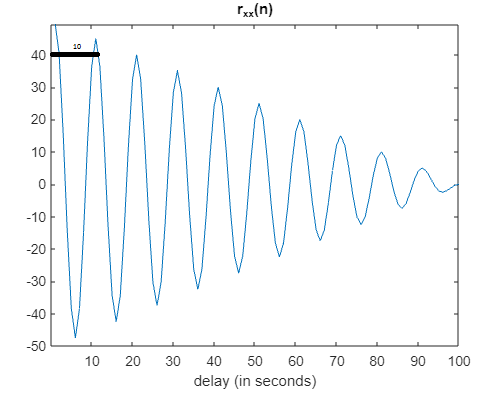
\includegraphics[width=\textwidth]{Untitled1.png}
		\caption{Auto- correlation of Sin wave}
	\end{subfigure}
\end{figure1}



\ sample rate = 100

\ The auto correlation function of $x(n)$ 


\ as we can see that there are regions of maximum peaks , from here we will find the difference between the maximum peak and the second peak which comes out to be 10 sec and it is the pitch period.

\begin{equation} Pitch =  \frac{sample Rate}{Period}   \end{equation}

\ After putting the value the pitch =10 Hz which is indeed the fundamental frequency of signal
Note that autocorellation function gives maximum peak at zero lag. Since the speech signal at this delay is replication of itself. As we have to find the next maximum peak and measure the number of sample.
\subsection{Assumptions}

\ For the proper working of this PDA (Pitch Detection Algorithm ) we have taken those Frame as the voiced frame where the energy of frame is greater then or equal to the average energy of whole frame else we consider it as unvoiced frame.Although it is not good way to segment the frame as many time the unvoiced frame also get considered as voiced frame. 
\subsection{Algorithms used}

\ Working of the Pitch Detection Algorithm can be understood from following:

\begin{itemize}
  \item read the sound wave from the user.
  \item Now divide the whole sound wave into small overlapping or non-overlapping frames using winSize and hoplen
  \item Now perform the segmentation of speech signal into viced and unvoiced frame
  \item for voiced frame perform auto-correlation and return the estimated pitch
  \item for unvoiced frame return zero
\end{itemize}

\section{Results and analysis}
\ Let Try our algorithm on different voiced frame and unvoiced frames , results are added at the end of the this report.
\\ \textbf{Observation}

\begin{itemize}
  \item For Voiced Frame the maximum peak at the zero delay as expected
  \item Some time unvoiced frame and voiced frame are not properly segmented i.e energy based segmentation not always works well.
  \item If we take ACF of unvoiced frame we don't get regions of maxima's that we get in case of voiced.
\end{itemize}
\begin{figure}[h]
	\centering
	\begin{subfigure}
		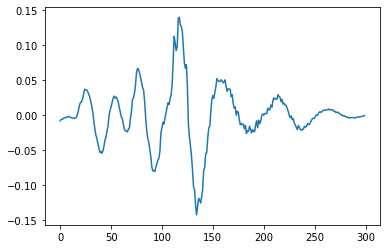
\includegraphics[width=\textwidth]{true1frame.png}
		\caption{Voiced Frame}
	\end{subfigure}
	\begin{subfigure}
		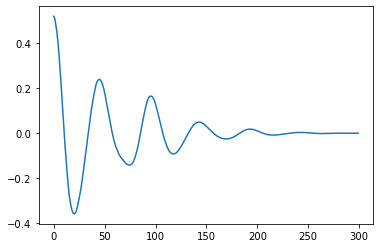
\includegraphics[width=\textwidth]{True1auto.png}
		\caption{Auto- correlation of Voiced Frame Pitch = 222.2 Hz}
	\end{subfigure}
\end{figure}

\begin{figure}[h]
	\centering
	\begin{subfigure}
		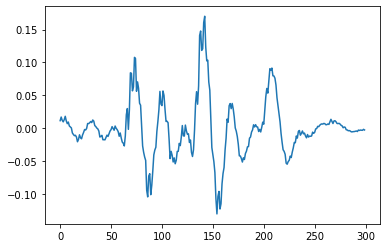
\includegraphics[width=\textwidth]{true2frame.png}
		\caption{Voiced Frame}
	\end{subfigure}
	\begin{subfigure}
		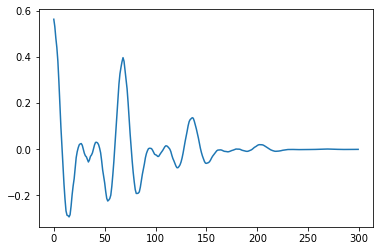
\includegraphics[width=\textwidth]{True2auto.png}
		\caption{Auto- correlation of Voiced Frame Pitch = 147.05 Hz}
	\end{subfigure}
\end{figure}

\begin{figure}[h]
	\centering
	\begin{subfigure}
		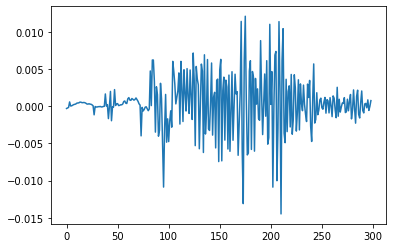
\includegraphics[width=\textwidth]{Fail1frameR.png}
		\caption{unvoiced Frame Detected}
	\end{subfigure}
	\begin{subfigure}
		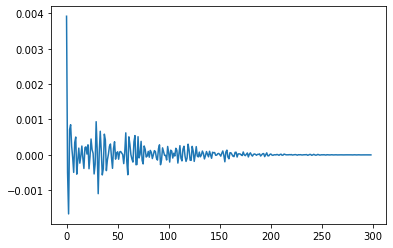
\includegraphics[width=\textwidth]{fail1frame.png}
		\caption{Auto- correlation of unvoiced Frame }
	\end{subfigure}
\end{figure}


\begin{figure}[h]
	\centering
	\begin{subfigure}
		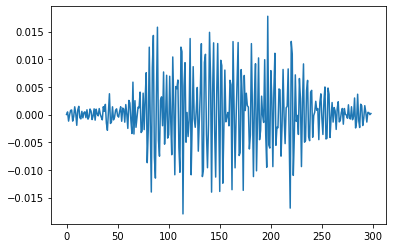
\includegraphics[width=\textwidth]{Fail2frameR.png}
		\caption{unvoiced Frame}
	\end{subfigure}
	\begin{subfigure}
		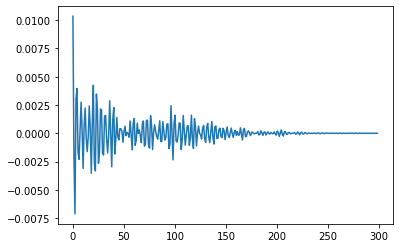
\includegraphics[width=\textwidth]{fail2frame.png}
		\caption{Auto- correlation of unvoiced Frame}
	\end{subfigure}
\end{figure}


\section{Conclusion}
\ The results that we got are quite interesting we saw that how a simple correlation function can be used to determine the pitch and how to segment the speech based on the energy present in each frame.
\ As we have seen from the results that algorithm preform well even though we are using a naive approach given that we have properly segmented the voiced and unvoiced frame. 
\section{Project Github page}
\url{https://github.com/rjn32s/pitch-Estimation-t21016} 

\section{References}


% uncomment these to generate the biblography

%\setstretch{1}
%\bibliographystyle{IEEEtran}
%\bibliography{mybib}

\end{document}